% Created by tikzDevice version 0.6.2-92-0ad2792 on 2013-02-14 18:25:26
% !TEX encoding = UTF-8 Unicode
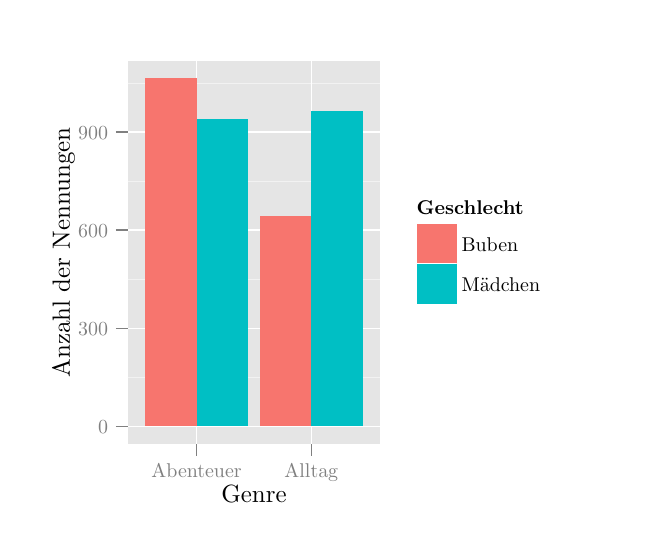
\begin{tikzpicture}[x=1pt,y=1pt]
\definecolor[named]{fillColor}{rgb}{1.00,1.00,1.00}
\path[use as bounding box,fill=fillColor,fill opacity=0.00] (0,0) rectangle (216.81,180.67);
\begin{scope}
\path[clip] (  0.00,  0.00) rectangle (216.81,180.67);
\definecolor[named]{drawColor}{rgb}{1.00,1.00,1.00}
\definecolor[named]{fillColor}{rgb}{1.00,1.00,1.00}

\path[draw=drawColor,line width= 0.6pt,line join=round,line cap=round,fill=fillColor] (  0.00,  0.00) rectangle (216.81,180.67);
\end{scope}
\begin{scope}
\path[clip] ( 36.15, 30.32) rectangle (127.38,168.63);
\definecolor[named]{fillColor}{rgb}{0.90,0.90,0.90}

\path[fill=fillColor] ( 36.15, 30.32) rectangle (127.38,168.63);
\definecolor[named]{drawColor}{rgb}{0.95,0.95,0.95}

\path[draw=drawColor,line width= 0.3pt,line join=round] ( 36.15, 54.31) --
	(127.38, 54.31);

\path[draw=drawColor,line width= 0.3pt,line join=round] ( 36.15, 89.73) --
	(127.38, 89.73);

\path[draw=drawColor,line width= 0.3pt,line join=round] ( 36.15,125.15) --
	(127.38,125.15);

\path[draw=drawColor,line width= 0.3pt,line join=round] ( 36.15,160.57) --
	(127.38,160.57);
\definecolor[named]{drawColor}{rgb}{1.00,1.00,1.00}

\path[draw=drawColor,line width= 0.6pt,line join=round] ( 36.15, 36.60) --
	(127.38, 36.60);

\path[draw=drawColor,line width= 0.6pt,line join=round] ( 36.15, 72.02) --
	(127.38, 72.02);

\path[draw=drawColor,line width= 0.6pt,line join=round] ( 36.15,107.44) --
	(127.38,107.44);

\path[draw=drawColor,line width= 0.6pt,line join=round] ( 36.15,142.86) --
	(127.38,142.86);

\path[draw=drawColor,line width= 0.6pt,line join=round] ( 61.03, 30.32) --
	( 61.03,168.63);

\path[draw=drawColor,line width= 0.6pt,line join=round] (102.50, 30.32) --
	(102.50,168.63);
\definecolor[named]{fillColor}{rgb}{0.97,0.46,0.43}

\path[fill=fillColor] ( 42.37, 36.60) rectangle ( 61.03,162.34);
\definecolor[named]{fillColor}{rgb}{0.00,0.75,0.77}

\path[fill=fillColor] ( 61.03, 36.60) rectangle ( 79.69,147.70);
\definecolor[named]{fillColor}{rgb}{0.97,0.46,0.43}

\path[fill=fillColor] ( 83.84, 36.60) rectangle (102.50,112.76);
\definecolor[named]{fillColor}{rgb}{0.00,0.75,0.77}

\path[fill=fillColor] (102.50, 36.60) rectangle (121.16,150.42);
\end{scope}
\begin{scope}
\path[clip] (  0.00,  0.00) rectangle (216.81,180.67);
\definecolor[named]{drawColor}{rgb}{0.50,0.50,0.50}

\node[text=drawColor,anchor=base east,inner sep=0pt, outer sep=0pt, scale=  0.72] at ( 29.04, 34.12) {0};

\node[text=drawColor,anchor=base east,inner sep=0pt, outer sep=0pt, scale=  0.72] at ( 29.04, 69.54) {300};

\node[text=drawColor,anchor=base east,inner sep=0pt, outer sep=0pt, scale=  0.72] at ( 29.04,104.96) {600};

\node[text=drawColor,anchor=base east,inner sep=0pt, outer sep=0pt, scale=  0.72] at ( 29.04,140.38) {900};
\end{scope}
\begin{scope}
\path[clip] (  0.00,  0.00) rectangle (216.81,180.67);
\definecolor[named]{drawColor}{rgb}{0.50,0.50,0.50}

\path[draw=drawColor,line width= 0.6pt,line join=round] ( 31.89, 36.60) --
	( 36.15, 36.60);

\path[draw=drawColor,line width= 0.6pt,line join=round] ( 31.89, 72.02) --
	( 36.15, 72.02);

\path[draw=drawColor,line width= 0.6pt,line join=round] ( 31.89,107.44) --
	( 36.15,107.44);

\path[draw=drawColor,line width= 0.6pt,line join=round] ( 31.89,142.86) --
	( 36.15,142.86);
\end{scope}
\begin{scope}
\path[clip] (  0.00,  0.00) rectangle (216.81,180.67);
\definecolor[named]{drawColor}{rgb}{0.50,0.50,0.50}

\path[draw=drawColor,line width= 0.6pt,line join=round] ( 61.03, 26.05) --
	( 61.03, 30.32);

\path[draw=drawColor,line width= 0.6pt,line join=round] (102.50, 26.05) --
	(102.50, 30.32);
\end{scope}
\begin{scope}
\path[clip] (  0.00,  0.00) rectangle (216.81,180.67);
\definecolor[named]{drawColor}{rgb}{0.50,0.50,0.50}

\node[text=drawColor,anchor=base,inner sep=0pt, outer sep=0pt, scale=  0.72] at ( 61.03, 18.24) {Abenteuer};

\node[text=drawColor,anchor=base,inner sep=0pt, outer sep=0pt, scale=  0.72] at (102.50, 18.24) {Alltag};
\end{scope}
\begin{scope}
\path[clip] (  0.00,  0.00) rectangle (216.81,180.67);
\definecolor[named]{drawColor}{rgb}{0.00,0.00,0.00}

\node[text=drawColor,anchor=base,inner sep=0pt, outer sep=0pt, scale=  0.90] at ( 81.77,  9.03) {Genre};
\end{scope}
\begin{scope}
\path[clip] (  0.00,  0.00) rectangle (216.81,180.67);
\definecolor[named]{drawColor}{rgb}{0.00,0.00,0.00}

\node[text=drawColor,rotate= 90.00,anchor=base,inner sep=0pt, outer sep=0pt, scale=  0.90] at ( 15.23, 99.47) {Anzahl der Nennungen};
\end{scope}
\begin{scope}
\path[clip] (  0.00,  0.00) rectangle (216.81,180.67);
\definecolor[named]{fillColor}{rgb}{1.00,1.00,1.00}

\path[fill=fillColor] (136.25, 76.46) rectangle (195.90,122.49);
\end{scope}
\begin{scope}
\path[clip] (  0.00,  0.00) rectangle (216.81,180.67);
\definecolor[named]{drawColor}{rgb}{0.00,0.00,0.00}

\node[text=drawColor,anchor=base west,inner sep=0pt, outer sep=0pt, scale=  0.72] at (140.52,113.25) {\bfseries Geschlecht};
\end{scope}
\begin{scope}
\path[clip] (  0.00,  0.00) rectangle (216.81,180.67);
\definecolor[named]{drawColor}{rgb}{1.00,1.00,1.00}
\definecolor[named]{fillColor}{rgb}{0.95,0.95,0.95}

\path[draw=drawColor,line width= 0.6pt,line join=round,line cap=round,fill=fillColor] (140.52, 95.18) rectangle (154.97,109.64);
\end{scope}
\begin{scope}
\path[clip] (  0.00,  0.00) rectangle (216.81,180.67);
\definecolor[named]{fillColor}{rgb}{0.97,0.46,0.43}

\path[fill=fillColor] (140.52, 95.18) rectangle (154.97,109.64);

\path[] (140.52, 95.18) --
	(154.97,109.64);
\end{scope}
\begin{scope}
\path[clip] (  0.00,  0.00) rectangle (216.81,180.67);
\definecolor[named]{drawColor}{rgb}{1.00,1.00,1.00}
\definecolor[named]{fillColor}{rgb}{0.95,0.95,0.95}

\path[draw=drawColor,line width= 0.6pt,line join=round,line cap=round,fill=fillColor] (140.52, 80.73) rectangle (154.97, 95.18);
\end{scope}
\begin{scope}
\path[clip] (  0.00,  0.00) rectangle (216.81,180.67);
\definecolor[named]{fillColor}{rgb}{0.00,0.75,0.77}

\path[fill=fillColor] (140.52, 80.73) rectangle (154.97, 95.18);

\path[] (140.52, 80.73) --
	(154.97, 95.18);
\end{scope}
\begin{scope}
\path[clip] (  0.00,  0.00) rectangle (216.81,180.67);
\definecolor[named]{drawColor}{rgb}{0.00,0.00,0.00}

\node[text=drawColor,anchor=base west,inner sep=0pt, outer sep=0pt, scale=  0.72] at (156.78, 99.93) {Buben};
\end{scope}
\begin{scope}
\path[clip] (  0.00,  0.00) rectangle (216.81,180.67);
\definecolor[named]{drawColor}{rgb}{0.00,0.00,0.00}

\node[text=drawColor,anchor=base west,inner sep=0pt, outer sep=0pt, scale=  0.72] at (156.78, 85.48) {Mädchen};
\end{scope}
\end{tikzpicture}
